

% DOCUMENT CLASS  ================================
\documentclass[12pt, a4paper]{article}              % document class


% PACKAGES =======================================

% Encoding ---------------------------------------
\usepackage[utf8]{inputenc}                         % unicode 
% Math -------------------------------------------
\usepackage[fleqn]{amsmath}
\usepackage{amssymb}
\usepackage{mathtools}

% Language ---------------------------------------
\usepackage[ngerman]{babel}                         % german text

% Page Format ------------------------------------
\usepackage{a4wide}                                 % page borders
\usepackage{lscape}                                 % landscape

% Text Format ------------------------------------
\usepackage{enumitem}                               % items in enumerate

% Figures and Tables -----------------------------
\usepackage{tabularx}                               % tables with variable column with
\usepackage{longtable}                              % tables with page break
\usepackage{booktabs}
\usepackage{wrapfig}

% Graphics ---------------------------------------
\usepackage{graphicx}
\usepackage[pdftex]{hyperref}                       % hyperlinks in PDF
\usepackage{color}
\usepackage[dvipsnames]{xcolor}
\usepackage{tikz}

% Misc -------------------------------------------
\usepackage{url}                                    % web links
\usepackage{listings}                               % program listings
\usepackage{units}
% ================================================



% STYLE ==========================================

% Font family ------------------------------------
\renewcommand{\familydefault}{\sfdefault}           % sans serif as default

%  Color -----------------------------------------
\definecolor{lightgray}{cmyk}{0,0,0,0.3}

% PDF metadata -----------------------------------
\hypersetup{
  pdfauthor={Sebastian Domaschke},
  pdftitle={\"Ubung FEM: Galerkin}
}

% ================================================


% PAGE FORMAT ====================================

% Typesetting ------------------------------------
\setlength{\textheight}{245mm}                      % text height
\setlength{\topmargin}{-15mm}                       % top margin
\setlength{\parindent}{0mm}                          

% ================================================


% TIKZ ===========================================

\usetikzlibrary{%
  arrows,%
  patterns,%
  decorations.pathmorphing,%
  decorations.markings,%
  decorations.pathreplacing,%
  shapes.symbols%
}

% ================================================


% MACROS =========================================

\newcommand*\circled[1]{\tikz[baseline=(char.base)]{
  \node[shape=circle,draw,inner sep=2pt] (char) {#1};}}

% Math -------------------------------------------
\def\v#1{\boldsymbol{#1}}                           % vector
\def\e{\mathrm{e}}                                  % Eulers number
\def\j{\mathrm{j}}                                  % complex unit
\def\d{\mathrm{d}}                                  % differential operator
\def\const{\mathrm{const}}                          % constant value

% Web --------------------------------------------
\def\email#1{%
  \href{mailto:#1}{%
    \expandafter\nolinkurl\expandafter{#1}%
  }%
}

% ================================================


\begin{document}


\thispagestyle{empty}
\begin{figure}[h!]
\centering

\includegraphics[scale=0.57]{Logo.png}
\end{figure}



\begin{minipage}[t]{0.72\textwidth}
  \textbf{\Huge Übung FEM: Galerkin}\\[.7ex]
\end{minipage}
\hfill
\begin{minipage}[t]{0.25\textwidth}
  %\raggedleft
  %
\includegraphics[width=\linewidth]{logo.pdf}
\end{minipage}



\section*{Einleitung}
In dieser Übung bestimmen Sie mit der Galerkin-Methode Näherungslösungen für das Verschiebungsfeld $u(x)$ eines eindimensionalen Stabs.



\section*{Stab mit Linienlast}

Der Stab der Länge~$L$ ist wie abgebildet rechtsseitig eingespannt mit einer vorgegegebenen Verschiebung~$\bar{u}_L \neq 0$.
Sowohl Querschnitt~$A$ als auch E-Modul~$E$ seien konstant.
Über der Stab\-länge verteilt wirkt die axiale Linienlast $n(x)=\nu\,A\,x^2$ und zusätzlich links die Zugspannung~$\bar{t}_0$.
Die schwache Form des Gleichgewichts ist in~\eqref{eqn:Weak} gegeben.

\bigskip

\begin{minipage}[t]{.43\textwidth}
  \subsubsection*{System}
  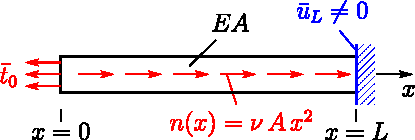
\includegraphics[]{truss}
\end{minipage}
\hfill
\begin{minipage}[t]{.51\textwidth}
  \subsubsection*{Schwache Form des Gleichgewichts}
  \begin{equation}\tag{$*$}\label{eqn:Weak}
  \begin{split}
    0 = & -\int_0^L \textcolor{Green}{g'(x)} \,EA \,u'(x) \,\d x \\
        & -\textcolor{Green}{g(0)} \, A \,\textcolor{Red}{\bar{t}_0} \\
        & +\int_0^L \textcolor{Green}{g(x)} \,\textcolor{Red}{\nu A \, x^2\,} \d x \qquad \forall \textcolor{Green}{g^\mathrm{vert}}
  \end{split}
  \end{equation}
\end{minipage}

\bigskip
\subsubsection*{Teil I: Näherungslösungen nach Galerkin (3 Varianten)}
Bestimmen Sie drei Näherungslösungen des Verschiebungsfelds $u(x)$ mit der Galerkin-Methode.
\paragraph{Teil 1a) Linearer Ansatz}
Führen Sie die folgenden 6 Schritte aus, um eine erste Näherungslösung zu bestimmen.
\begin{enumerate}[label=\protect\circled{\arabic*}]
  \item Als Ansatzfunktion \emph{wählen} wir eine lineare Funktion der Form
    \begin{equation}\label{eqn:Trial}
      u(x) = c_0 + c_1\,x
    \end{equation}
  \item Geben Sie die gemäss \emph{Galerkin} zu \eqref{eqn:Trial} passende Gewichtungsfunktion an
    \begin{equation}
       \textcolor{Green}{g_u(x) = } \label{eqn:Test}
    \end{equation}
  \item Werten Sie die \emph{Verschiebungsrandbedingung} aus um die Ansatzfunktion \eqref{eqn:Trial} zu vereinfachen
    \begin{align}
      \qquad = u(L) = \qquad\qquad & \Rightarrow \qquad &\Rightarrow \quad u(x) =  \label{eqn:TrialSimple}
    \end{align}
    \item Welche Bedingung muss die Gewichtungsfunktion~\eqref{eqn:Test} erfüllen, damit diese mit der Verschiebungsrandbedingung \emph{verträglich} ist? Vereinfachen Sie damit die Gewichtungsfunktion~\eqref{eqn:Test}
    \begin{align}
      \qquad \textcolor{Green}{ = g_u(L) = } \qquad\qquad & \Rightarrow  \qquad\qquad &\Rightarrow \quad  \textcolor{Green}{g_u(x) =} \label{eqn:TestSimple}
    \end{align}
  \item \emph{Differenzieren} Sie die vereinfachten Funktionen \eqref{eqn:TrialSimple} und \eqref{eqn:TestSimple} nach $x$
    \begin{align}
      u'(x) &=  \label{eqn:TrialPrime} \\[1em]
      \textcolor{Green}{g_u'(x)} & \textcolor{Green}{=} \label{eqn:TestPrime}
    \end{align}
   \item Nun sind Sie vorbereitet um~\eqref{eqn:Weak} auszuwerten. Bestimmen Sie durch Einsetzen von~\eqref{eqn:TrialSimple}--\eqref{eqn:TestPrime} die Konstante~$c_1$ und damit die Näherungslösung~$u(x)$
   \begin{equation}\label{eqn:Approximation}
     0 = 
   \end{equation}\vspace{4\baselineskip}
\end{enumerate}

\paragraph{Teil 1b) Quadratischer Ansatz}
Wiederholen Sie Teil 1a) mit einem quadratischen Ansatz
\begin{equation}\label{eqn:TrialQuad}
  u(x) = c_0 + c_1\,x + c_2\,x^2,
\end{equation}
und bestimmen Sie die unbekannten Koeffizienten aus der schwachen Form~\eqref{eqn:Weak}. %Achten Sie darauf, dass Ansatz- und Gewichtungsfunktionen mit der Verschiebungsrandbedingung $u(L)=\bar{u}_L$ verträglich sind.

 %\emph{Hinweis:} Beschreiben Sie die Ansatzfunktion nach Einarbeitung der Randbedingung sowie die Galerkin-Testfunktion mit den beiden Formfunktionen $N_1(x)=x-L$ und $N_2(x)=x^2-L^2$.\vspace{2\baselineskip}

\paragraph{Zusatz: Teil 1c) Trigonometrischer Ansatz}
Verwenden Sie als Ansatzfunktion die Form
\begin{equation}\label{eqn:TrialSin}
  u(x) = a_0 + a_1\,\sin\!\left(\frac{x}{L}\right).
\end{equation}
und bestimmen Sie die unbekannten Koeffizienten aus der schwachen Form~\eqref{eqn:Weak}. %Achten Sie darauf, dass Ansatz- und Gewichtungsfunktionen mit der Verschiebungsrandbedingung $u(L)=\bar{u}_L$ verträglich sind.
\\

\emph{Tipp:}
\begin{equation}
\int \cos^2(x/L)\,\mathrm{d}x=\frac{x}{2}+\frac{L}{4}\sin\!\left(\frac{2x}{L}\right)+C
\end{equation}
\begin{equation}
\int x^2\sin(x/L)\,\mathrm{d}x=-Lx^2\cos\!\left(\frac{x}{L}\right)+2L^2x\sin\!\left(\frac{x}{L}\right)+2L^3\cos\!\left(\frac{x}{L}\right)+C
\end{equation}




\newpage
\subsubsection*{Teil II: Vergleich (Näherung vs. analytisch)}
Die analytische Lösung zu~\eqref{eqn:Weak} lautet
  \begin{equation}\label{eqn:Solution}
    \hat{u}(x) = \bar{u}_L + \frac{t_0}{E}(x - L) - \frac{\nu}{12 E}(x^4 - L^4).
  \end{equation}

  Wie gut passen Ihre Näherungslösungen aus Teil 1a)--1c) zur analytischen Lösung~\eqref{eqn:Solution}?
  
  Für einen \emph{quantitativen Vergleich} verwenden Sie die folgenden Eingabewerte:
  \[
    E=10^5,\quad L=2,\quad \nu=1,\quad \bar{u}_L=0,\quad \bar{t}_0=10.
  \]
  Vergleichen Sie $u(x)$ und $\sigma(x)$ für die drei Ansätze im bereich  $x\in(0,L)$. Diskutieren Sie Ihre Erkenntnisse. \vspace{2\baselineskip}



\subsubsection*{Teil III: Theoretische Diskussion}
\begin{enumerate}[label=\protect\circled{\arabic*}]
  \item Für welche Gewichtungsfunktionen $\textcolor{Green}{g_{\hat{u}}(x)}$ erfüllt die Lösung~\eqref{eqn:Solution} die schwache Form des Gleichgewichts~\eqref{eqn:Weak}?\vspace{3\baselineskip}
  \item Für welche Gewichtungsfunktionen $\textcolor{Green}{g_u(x)}$ erfüllen Ihre Näherungslösungen aus Teil 1a)--1c) die schwache Form des Gleichgewichts~\eqref{eqn:Weak}?\vspace{3\baselineskip}
  \item Durch welche Massnahmen könnte die Näherungslösung verbessert werden? \vspace{3\baselineskip}
  \item Wie müssten Sie konkret in einer FEM-Software vorgehen, um die Näherungslösung zu verbessern? \vspace{3\baselineskip}
\end{enumerate}


\end{document}